\chapter{Background}
\lhead{Background}
\label{Background}

	\section{Related Work}
	\label{Background:RelatedWork}
	
		One of the main challenges of informative path planning include selecting the appropriate acquisition function suitable for the type of exploration task at hand. \textit{Acquisition functions}, or \textit{acquisition criterion}, measures the desirability of observing a particular location. In the informative path planning scenario, the acquisition function evaluates the amount of total information or uncertainty contained by a given candidate path. In this context, the way in which \textit{total information} is quantified determines the acquisition function. The more information the path contains, the more desirable it is for the AUV to follow and take observations on that path. 

		The effectiveness of an acquisition function that measures mutual information throughout a particular given path has been thoroughly investigated in the literature \citep{AsherBender, Rigby:ROB20372, Krause:2008:NSP:1390681.1390689, Kapoor}. \textit{Mutual information} refers to a measure of information that takes into account the overlapping information within the region or path in consideration. In most spatial sampling contexts, it is unlikely that two given locations within a region or path are completely unrelated or uncorrelated. Observations in one location provides partial information regarding other locations, which is the primary reason that an accurate benthic habitat map can be obtained without visiting all locations within the region exhaustively. Without considering mutual information, an agent such as an AUV may be prompted to observe locations that contain similar information, thus achieving inefficient mapping.
		
		Several types of acquisition functions have been proposed in the benthic habitat mapping context. \cite{AsherBender} uses an acquisition criterion given by \eqref{Equation:AsherBenderAcquisitionCriterion} where $\pi^{m}_{i}$ is the probability of the habitat label being a member of class $m \in \{1, \dots, c\}$ at query location $i \in \{1, \dots, n^{\star}\}$. Here $c$ is the number of classes and $n^{\star}$ is the number of query points.
		
		\begin{equation}
			H = - \frac{1}{n^{\star}} \sum_{i = 1}^{n^{\star}} \sum_{m = 1}^{c} \pi^{m}_{i} \log(\pi^{m}_{i})
		\label{Equation:AsherBenderAcquisitionCriterion}
		\end{equation}
		
		For a given query point $i$, $- \sum_{m = 1}^{c} \pi^{m}_{i} \log(\pi^{m}_{i})$ is exactly the prediction information entropy (PIE) at location $i$, which captures the local model uncertainty and thus potential information. As a result, the acquisition criterion given in \eqref{Equation:AsherBenderAcquisitionCriterion} is the mean of the marginalised PIE across query points, which does not capture mutual information through considering the joint distributions of the class labels across multiple query points $i \in \{1, \dots, n^{\star}\}$. This acquisition criterion will be referred to as MPIE for mean of marginalised prediction information entropy. In this approach, the quality of the habitat models are assessed by utility functions that evaluate the confidence of the GP classifier prediction, which is the difference of the MPIE before and after an observation is made \eqref{Equation:AsherBenderMutualInformationCriterion} \citep{Rigby:ROB20372}. This utility is used in conjunction with a GP classifier under probabilistic least squares approximation to optimise selected survey paths through considering the differential entropy across the entire region of interest (ROI). Below, $X, \bvec{y}$ are the observed feature locations and habitat labels, $X^{\star}$ to be the unobserved query locations, and $X_{p}, \bvec{y}_{p}$ are the observations made after traversing the proposed path.
	
		\begin{equation}
			I = H[X^{\star} | X, \bvec{y}] - H[X^{\star} | X \cup X_{p}, \bvec{y} \cup \bvec{y}_{p}]
		\label{Equation:AsherBenderMutualInformationCriterion}
		\end{equation}
		
		\cite{Krause:2008:NSP:1390681.1390689} instead focuses on sensor placement methodologies to optimse mutual information gained. This aims to reduce predictive variance at all query points. The chosen acquisition function is the difference between the MIE at all \textit{final} unobserved locations $X^{\star} \backslash X_{p}$ before and after the observations are taken \eqref{Equation:KrauseAcquisitionCriterion}.
		
		\begin{equation}
			I = H[X^{\star} \backslash X_{p} | X, \bvec{y}] - H[X^{\star} \backslash X_{p} | X \cup X_{p}, \bvec{y} \cup \bvec{y}_{p}]
		\label{Equation:KrauseAcquisitionCriterion}
		\end{equation}
		
		Under the GP classification model, however, this results in an integral that can only be estimated through sampling techniques which are computationally expensive. As such, computationally tractable methods usually employ experimental design philosophies in minimising the predictive variance \citep{AsherBender}.
		
		\cite{Kapoor} demonstrates the use of posterior mean and covariance of the GP classifier latent function. While this approach takes full advantage of the analytical forms available for a Gaussian latent process, it does not consider the mutual behaviour of the unobserved locations with the proposed path.
		
		On the other hand, \cite{Roman:SequentialBayesianOptimisation} approaches the problem from a continuous path-planning perspective for UAVs in which two Gaussian processes are used - one to model the phenomenon and another to assess the quality of proposed paths. However, this layered Sequential Bayesian Optimisation approach is primarily devised for a regression setting which becomes intractable when performed in the classification domain.
		
		Much of the intractability discussed in such literature can trace its reason down to the fact that benthic habitat mapping is a classification problem instead of a regression problem. While Gaussian process regression provide analytical forms for inference, due to a non-Gaussian likelihood response, Gaussian process classification is no longer analytically tractable. Instead, several approximations must be made, which is discussed in section \ref{Background:GaussianProcesses:Classification}.
		
		This thesis addresses the tractability status of the problem through proposing an alternative acquisition criterion, hereby named linearised model differential entropy (LMDE), that captures mutual information. In the current literature, acquisition criterion either do not directly capture mutual information, such as \eqref{Equation:AsherBenderAcquisitionCriterion}, or take too long to compute due to required estimations from sampling, such as \eqref{Equation:KrauseAcquisitionCriterion}. This work shows that LMDE as an acquisition function captures an appropriate form of mutual information. Furthermore, LDME outperforms other acquisitions in both ractability and mapping accuracy.
		
	\section{Gaussian Processes}
	\label{Background:GaussianProcesses}
	
		Gaussian processes (GP) are stochastic processes which generalises the multi-variate Gaussian distribution. In a statistical learning and machine learning context, they are categorised as a type of \textit{supervised learning} method, which describes the problem of learning relationships between input and output variables from empirical data. The empirical data is also often referred to as the training set.
		
		Supervised learning methods are further categorised into regression and classification problems, depending on the nature of the output variable. The problem is a regression problem if the output is continuous, and a classification problem if the output is discrete. For example, when bathymetric feature extraction is analytically infeasible, bathymetric modeling becomes a regression problem, where the output variables are the bathymetric features. A common instance of the bathymetric modeling problem is seafloor depth modeling, in which the terrain elevation structure is the continuous output to be inferred. Benthic habitat mapping, on the other hand, involves inference of discrete habitat labels and is thus a classification problem.
		
		In both regression and classification settings, the input variables are often also referred to as \textit{features}, which motivated the term \textit{bathymetric features} in the previous sections. This also helps to distinguish the features from the spatial inputs, which are not necessarily the input variables involved in the supervised learning problem. In statistical literature, continuous regression outputs are sometimes called \textit{response} variables, although it is more often simply referred as the \textit{output} or \textit{target} in the machine learning community. However, in the Gaussian process classification setting, the term \textit{response} also refers to the likelihood response involved in the model. Therefore, the use of the term \textit{response} will be reserved for the latter in this thesis. Discrete classification outputs are often referred to as \textit{labels}, although the term \textit{target} is also used. In the benthic habitat mapping context, the type of henthic habitats are the labels to be inferred or predicted. 
		
		In the sections which references the use of Gaussian process models, $\bvec{x}$ will denote the input variable or features of the problem while $y$ will denote the output or target variable. Note that in general there are multiple features such that the input is a feature vector $\bvec{x}$. Without loss of generality, however, the output variable can always be treated as a scalar quantity $y$. Under cases of multiple output variables, the problem can be split into multiple single output variable problems.
		
		%%% If I need to talk about multi-task regressoin, put it in the appendix and put a note here saying that I can expand on this more.
		
		% It is true that prediction performance may be improved by considering the output vector together, which leads to multi-task regression, as will be briefly discussed. However, this is only the case if the training features the multiple outputs are located in different parts of the feature space, which does not occur for 

		The work presented here will be primarily based on \textit{Gaussian Process for Machine Learning} by \cite{GaussianProcessForMachineLearning}. 

		\subsection{Bayesian Modeling with Gaussian Processes}
		\label{Background:GaussianProcesses:BayesianModeling}
		
			The Gaussian process formulation follows the Bayesian modeling philosophy. An important distinction Bayesian modeling makes from the classical approach is the idea of estimating a distribution instead of a point value. While this is often more computationally expensive, it provides a very robust and accurate framework for prediction and inference. More importantly, it provides capabilities that classical approaches do not possess - the ability to quantify prediction uncertainties and, most importantly, potential information. 
			
			Suppose $H$ represents the event that a particular inference model $\mathcal{H}$ is representative of the true underlying phenomenon to be inferred. Further suppose $D$ represents the event that a particular set of observations $\mathcal{D}$ have been collected. The basic Bayesian modeling process begins with a \textit{prior} distribution $p(H)$, the probability of $\mathcal{H}$ being representative before $\mathcal{D}$ was observed, and updates this to a \textit{posterior} distribution $p(H | D)$, the updated probability of $\mathcal{H}$ being representative after observing $\mathcal{D}$. In this way, $\mathcal{H}$ can be interpreted as the agent's belief of the phenomenon. In the benthic habitat mapping context, the agent is the AUV, and the phenomenon is the type of benthic habitats distributed about the region of interest.
			
			In general, this belief update is achieved through Bayes theorem \eqref{Equation:Bayes}. The \textit{likelihood} distribution $p(D | H)$ is the probability of observing the dataset $\mathcal{D}$ given that $\mathcal{H}$ is representative of the true underlying phenomenon. The \textit{evidence} distribution $p(D)$ is the probability of observing the dataset. However, in practice it is often difficult to compute the evidence without a model. Hence, expanding over all possible inference models $\mathcal{H}$, the evidence can also be found by marginalising the joint distribution $p(D \cap H) = p(D | H) p(H)$ of observing $\mathcal{D}$ and $\mathcal{H}$ being representative \eqref{Equation:MarginalLikelihood}. In this way, the evidence is also referred to as the \textit{marginal likelihood}.
			
			\begin{equation}
				p(H | D) = \frac{p(D | H) p(H)}{p(D)} \qquad \Longleftrightarrow \qquad \mathrm{posterior} = \frac{\mathrm{likelihood} \times \mathrm{prior}}{\mathrm{evidence}}
			\label{Equation:Bayes}
			\end{equation}
			
			\begin{equation}
				p(D) = \sum_{H} p(D | H) p(H)
			\label{Equation:MarginalLikelihood}
			\end{equation}			
			
			This procedure is illustrated in \cref{Figure:BayesianModeling} for a Gaussian process with one dimensional input feature and output target, where the prior is updated into a posterior after two observations. This example further serves to illustrate the concept of distributions over functions, which behaves as an infinite dimensional generalisation of a multivariate probability distribution. It is helpful to conceptualise functions as an infinite string of points, where functions can be interpreted as infinite dimensional vectors, such that drawing from an infinite dimensional distribution is equivalent to drawing from processes that operate on function space. Instead of drawing finite dimensional random vectors from distributions, a random function is drawn from a \textit{stochastic process} \footnote{When the input variable is temporal, a stochastic process can be more appropriately interpreted as having indefinite dimensional distributions.}.
			
			\begin{figure}[!htbp]
				\centering
					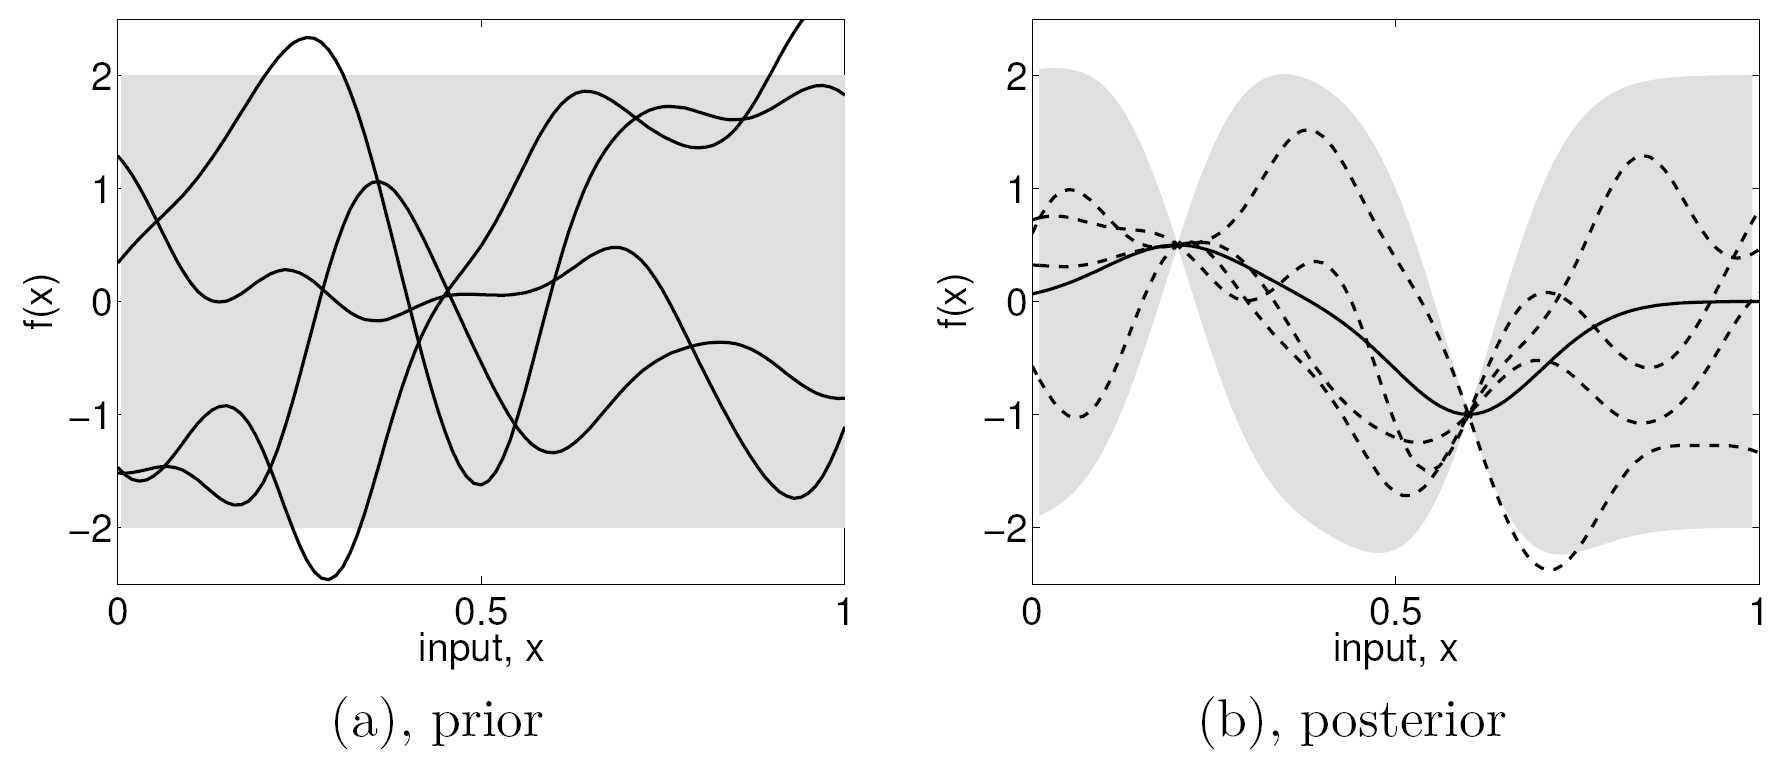
\includegraphics[width=0.9\textwidth]{Figures/bayesianmodeling.png}
				\caption{Illustration of Gaussian Process Bayesian Modeling: The mean prediction is shown as the solid line. Four samples are drawn in each case, represented by the dashed line. The shared region represents the 2-$\sigma$ bounds of the prediction at each input feature value $x$. Two points are observed which updated the distribution from the prior to the posterior.\\
				Figure (a) shows the situation for the prior distribution.\\
				Figure (b) shows the situation for the posterior distribution. \\
				Adapted from \cite{GaussianProcessForMachineLearning}}
				\label{Figure:BayesianModeling}
			\end{figure}
			
			From this illustration, there are a few qualities one can notice. Firstly, the prior distribution is simply the zero function. The prior is meant to represent the system's current belief before the next observations are to be made. In this case, the prior situation involves no observations at all. Ideally, this means that the prior distribution should contain no predictive information. However, it is of philosophical note that all informative \footnote{It is certainly possible to perform inference without any assumptions. It will simply be uninformative in prediction or result.} inferences must begin with some assumptions regarding the structure of the phenomenon to be inferenced. In the illustration above, the function is assumed to be distributed as a process with zero mean. This assumption has excluded processes without means, such as the Cauchy process, as well as assumed a rather arbitrary mean function. However, this assumption is often valid as one can always pre-process the output data set through subtracting off their empirical mean so that the output is approximately distributed about zero. The representation of the standard deviation and hence variance as confidence bounds centred at the mean function also means that multi-model processes are excluded. For a Gaussian process, which is indeed uni-modal and have finite moments for all moments of finite degree, this illustration is common and useful for visualising the Bayesian modeling process. It is customary to visualise the 2-$\sigma$ bound for a Gaussian process. So, for this example, the prior distribution has a uniform standard deviation of one everywhere.
			
			Regarding the variance, a second observation is that the standard deviation and hence variance of the output function decreases at the observations, and gradually increases away from the observations. This leads to two remarks. Firstly, the variance or uncertainty of the output function at a location reduces when observations are made at that location. Secondly, neighboring points are related - the closer they are, the more related they are. This is seen through the observed points dragging nearby points towards it while reducing the uncertainty of nearby points. This resembles the concept of covariance. Evidently, points closer to each other have higher covariance then those further away, and the covariance beween the same points simply become its variance.
			
			The two observations above demonstrate that, just as a Gaussian distribution is defined through a mean vector and a covariance matrix, a Gaussian process is defined through a mean function $m(x)$ and a covariance function $k(x, x')$. In Gaussian process literature, the covariance function is also called a \textit{kernel} function.
			
			With an intuition of Gaussian processes in the Bayesian modeling context, a formal definition of Gaussian processes can now be introduced. In this thesis, the shorthand notation $I_{n} := \{1, 2, \dots, n\}$ will be used for concise indexing unless otherwise indicated, and is not to be confused with identity matrices $I_{p \times p} \in \mathbb{R}^{p \times p}$.
			
			\newtheorem{gpdef}{Gaussian Process}[section]
			\begin{gpdef}
				A random function $f(x)$, $x \in \mathbb{R}$, is distributed as a Gaussian process with mean function $m(x)$ and covariance function $k(x, x')$, if for any finite collection of feature points $\bvec{x} := [x_{1}, x_{2}, \dots, x_{n}]^{T}$, the corresponding output targets $\bvec{f}(\bvec{x}) := \{f(x_{i})\}_{i \in I_{n}} := [f(x_{1}), f(x_{2}), \dots, f(x_{n})]^{T}$ is jointly multivariate Gaussian distributed such that 

					\begin{equation}
						\bvec{f}(\bvec{x}) \sim \mathcal{N}(\bvec{m}(\bvec{x}), K(\bvec{x}, \bvec{x}'))
					\label{Equation:GaussianProcessFiniteDistribution}
					\end{equation}	
				
				where $\bvec{m}(\bvec{x}) :=  \{m(x_{i})\}_{i \in I_{n}} \in \mathbb{R}^{n}$ and $K(\bvec{x}, \bvec{x}') := \{k(x_{i}, x_{j})\}_{i \in I_{n}, j \in I_{n}}$. Such a function $f(x)$ is then notated as
				
					\begin{equation}
						f(x) \sim \mathcal{GP}(m(x), k(x, x'))
					\label{Equation:GaussianProcess}
					\end{equation}	
					
			\label{Definition:GaussianProcess}
			\end{gpdef}
			
			Certainly, this definition generalises finite dimensional multivariate Gaussian distributions, in that any subset of a multivariate Gaussian distributed random vector is also a multivariate Gaussian distributed of lower dimensionality. Hence, 

			Definition \ref{Definition:GaussianProcess} is defined for a univariate input feature $x$. In fact, this definition generalises naturally to a multivariate input feature $\bvec{x} \in \mathbb{R}^{p}$ with $p$ features. This motivates definition \ref{Definition:GaussianRandomField}.
			
			\newtheorem{grfdef}{Gaussian Random Field}[section]
			\begin{grfdef}
				A random function $f(\bvec{x})$, $\bvec{x} \in \mathbb{R}^{p}$, is distributed as a Gaussian random field with mean function $m(\bvec{x})$ and covariance function $k(\bvec{x}, \bvec{x}')$, if for any finite collection of feature points $X := [\bvec{x}_{1}, \bvec{x}_{2}, \dots, \bvec{x}_{n}]^{T}$, the corresponding output targets $\bvec{f}(X) := \{f(\bvec{x}_{i})\}_{i \in I_{n}} := [f(\bvec{x}_{1}), f(\bvec{x}_{2}), \dots, f(\bvec{x}_{n})]^{T}$ is jointly multivariate Gaussian distributed such that 

					\begin{equation}
						\bvec{f}(X) \sim \mathcal{N}(\bvec{m}(X), K(X, X'))
					\label{Equation:GaussianRandomFieldFiniteDistribution}
					\end{equation}	
				
				where $\bvec{m}(X) :=  \{m(\bvec{x}_{i})\}_{i \in I_{n}} \in \mathbb{R}^{n}$ and $K(X, X') := \{k(\bvec{x}_{i}, \bvec{x}_{j})\}_{i \in I_{n}, j \in I_{n}}$. Such a function $f(\bvec{x})$ is then notated as
				
					\begin{equation}
						f(\bvec{x}) \sim \mathcal{GRF}(m(\bvec{x}), k(\bvec{x}, \bvec{x}'))
					\label{Equation:GaussianRandomField}
					\end{equation}	
					
			\label{Definition:GaussianRandomField}
			\end{grfdef}
			
			Notice that while Gaussian random fields describe the case for multivariate features, in practice the term is seldom used, and instead are also referred to as Gaussian processes. As such, it is conventional to simply write \eqref{Equation:GaussianRandomField} as \eqref{Equation:GaussianRandomFieldProcess}.
	
				\begin{equation}
					f(\bvec{x}) \sim \mathcal{GP}(m(\bvec{x}), k(\bvec{x}, \bvec{x}'))
				\label{Equation:GaussianRandomFieldProcess}
				\end{equation}	
							
			Finally, as mentioned before, the mean function can be generally assumed to be the zero function, as at each stage of inference both the model and data can be subtracted by their theoretical or empirical means. This elucidates that Gaussian processes are completely defined by their covariance function $k$. The covariance function $k$ is also refered to as the \textit{kernel} function. The next section will discuss the kernel function in detail.
			
			\FloatBarrier
			
		\subsection{Kernel Functions}
		\label{Background:GaussianProcesses:KernelFunctions}

			As kernel functions completely define the prediction and inference characteristics of a Gaussian process, this section aims to provide the mathematical background regarding kernels that are necessary for understanding Gaussian processes. The following discussion will only cover the minimal background necessary for further sections, as treatments of kernel functions can easily become very detailed and rigorous in topics such as differentiability effects or eigenfunction decomposition. Further treatment of this material is available through \cite{GaussianProcessForMachineLearning}. 
			
			Intuitively, the kernel function determines the \textit{similarity} between data points. This is a notion that all supervised learning algorithms intend to do, although rather implicitly in most cases. The GP formulation makes this explicit through the covariance between any two points in the feature space.
			
			Kernel functions can be categorised into stationary kernels and non-stationary kernels.
						
			\subsubsection{Stationary Kernels}
			\label{Background:GaussianProcesses:KernelFunctions:Stationary}
			
				Stationary kernels are ones whose covariance properties do not depend explicitly on the locations $\bvec{x}$ and $\bvec{x}'$ of consideration, but only on the difference $\bvec{x} - \bvec{x}'$ between them. Thus, the covariance properties are \textit{stationary}, or invariant, under translations in the feature space.
				
				Common stationary kernels are the squared exponential kernel \footnote{Squared exponential kernels are also sometimes called Gaussian kernels. However, in conversations it tends to create confusion between the probability density function $\phi(x)$ for Gaussian distributions and the covariance function $k(x, x')$ itself, so this term is avoided in this thesis.} and the \matern kernels, both of which belongs to the class of \textit{radial basis function} kernels. The squared exponential (SE) kernel between any two points $\bvec{x}, \bvec{x}' \in \mathbb{R}^{p}$ in the feature space with $p$ features has the following form \eqref{Equation:SquaredExponentialKernel}.
				
				\begin{equation}
					\left.
						\begin{aligned}
							k_{\mathrm{SE}}(\bvec{x}, \bvec{x}') &= \sigma_{f}^{2} \exp\Big(-\frac{1}{2}(\bvec{x} - \bvec{x}')^{T} \Sigma^{-1} (\bvec{x} - \bvec{x}')\Big) = \sigma_{f} \exp\Big(-\frac{1}{2} a^{2} \Big) \\
							\Sigma &= 	\begin{bmatrix}
											l_{1}^{2} & l_{12} & \dots & l_{1p} \\
											l_{21}^{2} & l_{2}^{2} & \dots & l_{2p} \\
											\vdots & \vdots  & \ddots & \vdots \\
											l_{p1}^{2} & l_{p2} & \dots & l_{p}^{2} \\
									  	\end{bmatrix}
						\end{aligned}
					\qquad \right.
				\label{Equation:SquaredExponentialKernel}
				\end{equation}
				
				Here, $\sigma_{f}$ is called the sensitivity, and determines the overall reference strength scale of the covariance function. The matrix $\Sigma$ is the length scale matrix, and determines the reference length scale and principle axis directions within the feature space. Like most quadratic forms, $\Sigma$ is required to be symmetric and positive semi-definite. In particular, when $\Sigma$ is diagonal, the kernel is termed \textit{axis aligned}. When $\Sigma$ is proportional to an identity such that $\Sigma = l^{2} I_{p \times p}$, the kernel is termed \textit{isotropic}.
				
				The sensitivity parameter $\sigma_{f}$ and length scale parameters $l_{ij}$, $i, j \in {1, 2, \dots, m}$ with $l_{i} := l_{ii}$ completely contain the information of a squared exponential kernel. Unlike parametric models, however, while these parameters define the kernel directly, they define the GP model indirectly. Because of the multiple levels of relation from these parameters to the model, these parameters are termed \textit{hyperparameters} of the GP.
				
				In practice, it is often possible to pre-process the data or transform the feature space so that an axis aligned kernel can be applied. The assumption imposed is that the principle axis directions are aligned with the feature space axis. In this case, the GP model is defined by $p + 1$ hyperparameters, where $p$ is the number of features. Without the axis-aligned structure, the number of hyperparameters is $\frac{p(p + 1)}{2} + 1$.
				
				The above formulation suggests to define $a^{2} := (\bvec{x} - \bvec{x}')^{T} \Sigma^{-1} (\bvec{x} - \bvec{x}')$. This can be interpreted as the squared distance between $\bvec{x}$ and $\bvec{x}'$ under the warp defined by $\Sigma$. In particular, when the feature space is isotropic such that $\Sigma = l^{2} I_{m \times m}$, then $a = \frac{r}{l}$ where $r := +\sqrt{r^{2}}$, $l := +\sqrt{l^{2}}$, and $r^{2} = (\bvec{x} - \bvec{x}')^{T} (\bvec{x} - \bvec{x}')$. In fact, most stationary kernels are functions solely of $a^{2}$, or with the definition $a := +\sqrt{a^{2}}$, they are simply scalar functions of scalar inputs $a = a (\bvec{x}, \bvec{x'})$. This form also makes evident that the covariances between two points decreases monotonically as the distance between them increases - a property most kernel functions exhibit. In fact, this structure characterises the \textit{radial basis function} class of kernels, and is the primary type of kernel relevant to this thesis.
				
				Continuing with this formulation, the \matern class of kernel functions are given by \eqref{Equation:MaternKernel}.
				
				\begin{equation}
					\left.
						\begin{aligned}
							k_{\mathrm{\maternmath}}(\bvec{x}, \bvec{x}') =& \; \sigma_{f}^{2} \frac{2^{1 - \nu}}{\Gamma(\nu)} \Big( \sqrt{2 \nu} a \Big)^{\nu} K_{\nu}\Big( \sqrt{2 \nu} a \Big) \\
							a^{2} :=& \; (\bvec{x} - \bvec{x}')^{T} \Sigma^{-1} (\bvec{x} - \bvec{x}')
						\end{aligned}
					\qquad \right.
				\label{Equation:MaternKernel}
				\end{equation}
							
				Here, $\Gamma$ and $K_{\nu}$ are the Gamma function and modified Bessel function respectively, while $\nu$ is a positive hyperparameter that determines the differentiability property of the \matern class kernel. The GP model with \matern class kernel is $d$-times mean square differentiable if and only if $\nu > d$ \citep{GaussianProcessForMachineLearning}. In the limit of $\nu \rightarrow \infty$ for infinite differentiability, the \matern kernel becomes the squared exponential kernel \eqref{Equation:SquaredExponentialKernel}. While the general \matern class kernel seem complicated due to the Gamma function and modified Bessel function, its form become simple for $\nu = p + \frac{1}{2}$ where $p$ is a non-negative integer. That is, \matern kernels with $\nu = \frac{1}{2}, \frac{3}{2}, \frac{5}{2}, \frac{7}{2}, \dots$ have simple analytic forms without reference to the modified Bessel function. In fact, for $\nu > \frac{5}{2}$, the degree for which the \matern kernel changes becomes quite unnoticeable for most practical purposes such that it may as well be replaced by the squared exponential kernel with $\nu \rightarrow \infty$. Similarly, while there is a more noticeable effect of changing $\nu$ within the range $\nu \in (0, \frac{5}{2})$, in practice is it is often not worth the expense of implementing the complicated form for a almost unnoticeable improvement in modeling accuracy. Hence, it is replaced with the \matern kernel with $\nu = \frac{1}{2}, \frac{3}{2}, \frac{5}{2}$, whichever is the closest. In this way, in practice only the \matern kernels with $\nu = \frac{1}{2}, \frac{3}{2}, \frac{5}{2}$ are employed, and they are respectively termed the \matern 1/2 kernel, \matern 3/2 kernel, and \matern 5/2 kernel - in the order of increasing differentiability. These kernels have the forms listed below \eqref{Equation:PracticalMaternKernels}.
				
				\begin{equation}
					\left.
						\begin{aligned}
							k_{\mathrm{\maternmath}, \; \nu = \frac{1}{2}}(\bvec{x}, \bvec{x}') =& \; \sigma_{f}^{2} \exp ( -a ) \\
							k_{\mathrm{\maternmath}, \; \nu = \frac{3}{2}}(\bvec{x}, \bvec{x}') =& \; \sigma_{f}^{2} (1 + \sqrt{3} a) \exp ( -\sqrt{3} a ) \\
							k_{\mathrm{\maternmath}, \; \nu = \frac{5}{2}}(\bvec{x}, \bvec{x}') =& \; \sigma_{f}^{2} \Big(1 + \sqrt{5} a + \frac{5}{3} a^{2}\Big) \exp ( -\sqrt{5} a )  \\
							a^{2} :=& \; (\bvec{x} - \bvec{x}')^{T} \Sigma^{-1} (\bvec{x} - \bvec{x}')
						\end{aligned}
					\qquad \right.
				\label{Equation:PracticalMaternKernels}
				\end{equation}			
				
				Together, the squared exponential kernel and the \matern class kernels provide a flexible set of kernel functions that can model a multitude of phenomena from various fields such as geology, ecology, finance, logistics, control theory, and machine learning.
			
			\subsubsection{Non-Stationary Kernels}
			\label{Background:GaussianProcesses:KernelFunctions:Nonstationary}
			
				Non-stationary kernels introduce flexibility for modeling phenomenons where the inherent length scales varies across feature locations. The limitations with stationary kernels is that the GP will always learn length scales that are as small as it needs to be for modeling the fastest varying phenomenon in the model. While the marginal likelihood inherently balances modeling accuracy and overfitting, when it comes to the choice between modeling a peak in data variation with a risk of overfitting the rest of the data or ignoring that peak, the optimiser will always prefer the former as marginal likelihood gain from successful modeling is higher than loss from overfitting. Because learning stage is done through optimising the marginal likelihood (see section \ref{Background:GaussianProcess:Regression:HyperparameterLearning}), this forces the length scale to be smaller than it needs at slower varying places.

				Figure \ref{Figure:GaussianProcessLengthScale} illustrates the non-stationary Gaussian process for a terrain modeling application. Note that this does not imply that it is only relevant for GP regression problems - the latent functions used in GP classification is itself a GP regression problem for which length scale interpretation is almost identical to that shown in \cref{Figure:GaussianProcessLengthScale} (see section \ref{Background:GaussianProcesses:Classification}).
				
				\begin{figure}[!htbp]
					\centering
						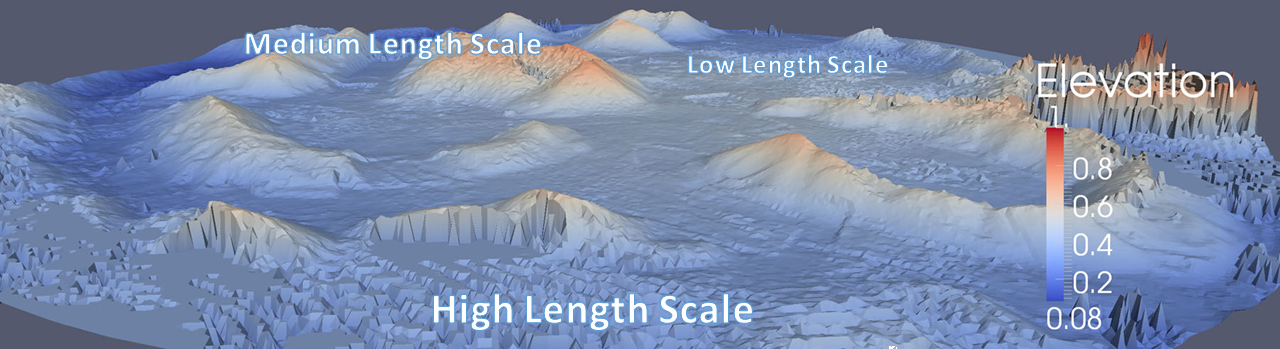
\includegraphics[width=\textwidth]{Figures/gaussianprocesslengthscale.png}
					\caption{Illustration of non-stationary Gaussian process for seafloor terrain modeling \citep{GaussianProcessTerrainFigure} \\
					Flat parts have high length scales (slow varying) while \\ rough parts have low length scales (fast varying)}
					\label{Figure:GaussianProcessLengthScale}
				\end{figure}
				
				The non-stationary kernel function employed in this thesis is the Paciorek non-stationary covariance kernel function \eqref{Equation:NonStationaryKernel} \citep{AdaptiveNonStationaryKernel}.
				
				\begin{equation}
					k(\bvec{x}_{i}, \bvec{x}_{j}) = \sigma_{f}^{2} |\Sigma_{i}|^{\frac{1}{4}} |\Sigma_{j}|^{\frac{1}{4}} \Bigg|\frac{\Sigma_{i} + \Sigma_{j}}{2}\Bigg|^{-\frac{1}{2}} \exp\Bigg[ -\frac{1}{2} (\bvec{x}_{i} - \bvec{x}_{j}) \Bigg(\frac{\Sigma_{i} + \Sigma_{j}}{2}\Bigg)^{-1} (\bvec{x}_{i} - \bvec{x}_{j}) \Bigg]
				\label{Equation:NonStationaryKernel}
				\end{equation}			
				
				The matrices $\Sigma_{i}$ and $\Sigma_{j}$ are the local length scale matrices at $\bvec{x}_{i}$ and $\bvec{x}_{j}$ respectively, and are interpreted the same way as the stationary case. The only difference is that these length scale matrices only operate locally, and are functions of the input feature vector $\bvec{x}$. In each kernel location, two length scale matrices are queried. Hence, in a kernel matrix of size $n \times m$, maximally $n + m$ unique queries are made if no feature locations overlap.
				
				It is worthwhile to observe that the effective length scale matrix in the exponent is the average of the two length scale matrices, with its effect reduced with increasing distance between the two points of consideration as with all kernels.
				
				Note that the normalisation matrix determinants are chosen such that the kernel function is reduced into the squared exponential stationary kernel when $\Sigma_{i} = \Sigma_{j} = \Sigma$, as derived in \eqref{Equation:NonStationaryKernelToStationaryKernel}. 
				
				\begin{equation}
					\left.
						\begin{aligned}
							k(\bvec{x}_{i}, \bvec{x}_{j}) &= \sigma_{f}^{2} |\Sigma|^{\frac{1}{4}} |\Sigma|^{\frac{1}{4}} \Bigg|\frac{\Sigma + \Sigma}{2}\Bigg|^{-\frac{1}{2}} \exp\Bigg[ -\frac{1}{2} (\bvec{x}_{i} - \bvec{x}_{j}) \Bigg(\frac{\Sigma + \Sigma}{2}\Bigg)^{-1} (\bvec{x}_{i} - \bvec{x}_{j}) \Bigg] \\
							k(\bvec{x}_{i}, \bvec{x}_{j}) &= \sigma_{f}^{2} |\Sigma|^{\frac{1}{2}} |\Sigma|^{-\frac{1}{2}} \exp\Bigg[ -\frac{1}{2} (\bvec{x}_{i} - \bvec{x}_{j}) (\Sigma)^{-1} (\bvec{x}_{i} - \bvec{x}_{j}) \Bigg] \\
							k(\bvec{x}_{i}, \bvec{x}_{j}) &= \sigma_{f}^{2} \exp\Bigg[ -\frac{1}{2} (\bvec{x}_{i} - \bvec{x}_{j}) \Sigma^{-1} (\bvec{x}_{i} - \bvec{x}_{j}) \Bigg]
						\end{aligned}
					\qquad \right.
				\label{Equation:NonStationaryKernelToStationaryKernel}
				\end{equation}		
				
				That is, the Paciorek non-stationary kernel reduces to the squared exponential kernel under the stationary limit. In this way, the Paciorek kernel generalises the squared exponential kernel.
				
				\FloatBarrier
			
		\subsection{Regression}
		\label{Background:GaussianProcesses:Regression}
		
			Gaussian process regression is a regression technique that employs Gaussian processes as its inference model. Because Gaussian processes already operate on function spaces with continuous inputs and outputs, no extra pre-processing or transformations are needed. The bulk of the technique thus lies in learning the kernel function of the Gaussian process. Gaussian process regression is also called \textit{kriging} or Kolmogorov Wiener prediction when used for interpolating geospatial data in a geostatistics setting. This section attempts to summarise the important concepts regarding GP regression and how they work. More rigorous discussions are available from \cite{GaussianProcessForMachineLearning}. 
			
			Once a kernel function is chosen, such as the squared exponential or \matern kernels, learning the kernel function becomes equivalent to learning the hyperparameters of the kernel. In this way, the Gaussian process model is actually defined completely by its hyperparameters. % , which are often only handful in quantity. % This illustrates that while its temporal complexity $\mathcal{O}(n^{3})$ is quite high, its spatial complexity and memory requirements are quite moderate at $\frac{m(m + 1)}{2} + 1 + n(m  + 1)$ real numbers, where $n(m  + 1)$ real numbers comes from the training data itself. % Minimally, after assuming a particular kernel functional form, the bulk of the model information is held by the data set itself. Especially in big data applications, unlike generalised linear models and neural networks whose information vector \footnote{The information vector is the vector of all parameters that defines the model.} is proportional to the number of basis functions employed, a Gaussian process model can have its information stored by a few hyperparameters.
			
			With a given kernel function $k$ as the covariance function, by definition \ref{Definition:GaussianRandomField} we have that the training observations $\bvec{f}$ and the query observations $\bvec{f^{\star}}$ is distributed as a multivariate Gaussian \eqref{Equation:InferenceJointDistribution}.
			
			\begin{equation}
				\begin{bmatrix}
					\bvec{f^{ }} \\ \bvec{f^{\star}}
				\end{bmatrix}
				\sim \mathcal{N}\Bigg(\bvec{0}, \begin{bmatrix}
													K(X, X) & K(X, X^{\star}) \\
													K(X^{\star}, X) & K(X^{\star}, X^{\star}) \\
												\end{bmatrix}  \Bigg)
			\label{Equation:InferenceJointDistribution}
			\end{equation}
			
			% where the matrix $K(X, X')$ is defined to have elements $K_{ij} = k(\bvec{x}_{i}, \bvec{x}'_{j})$ with $X$ and $X'$ defined as the canonical data design matrix form \eqref{Background:GaussianProcess:Equation:DataMatrix}, both of each can take either the matrix of training points $X$ of size $n$ or query points $X^{\star}$ of size $n^{\star}$.
			
			To shorten notation, it is customary to define $K := K(X, X)$, $K^{\star} := K(X, X^{\star})$, $K^{\star \star} := K(X^{\star}, X^{\star})$, where the symmetry of the covariance matrix readily yields ${K^{\star}}^{T} := K(X^{\star}, X)$. In this thesis, $K$ will be referred to as the \textit{data kernel} or \textit{training kernel}, $K^{\star}$ as the \textit{inference kernel}, and $K^{\star \star}$ as the \textit{query kernel}.
			
			\begin{equation}
				X = \begin{bmatrix}
					\bvec{x}_{1}^{T} \\ \bvec{x}_{2}^{T} \\ \dots \\ \bvec{x}_{n}^{T}
				\end{bmatrix} \qquad X' = \begin{bmatrix}
									\bvec{x'}_{1}^{T} \\ \bvec{x'}_{2}^{T} \\ \dots \\ \bvec{x'}_{n}^{T}
								\end{bmatrix}
			\label{Equation:TrainingQueryDataMatrices}
			\end{equation}	
				
			The joint distribution readily contains information for the conditional distribution of the query points given the training points $p(\bvec{f^{\star}} | \bvec{f})$ knowing the training points and query locations \footnote{Throughout this thesis, since the feature locations $X$ and $X^{\star}$ are always known, they are inherently conditioned upon and will not be shown explicitly in notation.}. This leads to the posterior distribution \eqref{Equation:InfereceConditionalDistribution}.
			
			\begin{equation}
				\bvec{f^{\star}} | \bvec{f} \sim \mathcal{N}({K^{\star}}^{T} K^{-1} \bvec{f}, K^{\star \star} - {K^{\star}}^{T} K^{-1} K^{\star})
			\label{Equation:InfereceConditionalDistribution}
			\end{equation}						
			
			A comparison with the prior $\bvec{f^{\star}} \sim \mathcal{N}(\bvec{0}, K^{\star \star})$ shows the mean effect ${K^{\star}}^{T} K^{-1} \bvec{f}$ and covariance effect $- {K^{\star}}^{T} K^{-1} K^{\star}$ which introduces observed information into the model. Interestingly, as ${K^{\star}}^{T} K^{-1} K^{\star}$ is positive definite, this intuitively means that the observation has reduced uncertainty in the model.
			
			The above posterior formulation encompasses the heart of the GP regression model. The rest of the discussion will focus on detailed aspects of its implementation and variants.
			
			% \subsubsection{Noisy Observations}
			
			Under noisy observations, a hyperparameter $\sigma$ is introduced for the standard deviation of the noise, which is also assumed to be \textit{iid} and Gaussian distributed with standard deviation $\sigma$ and zero mean. The only alteration is the observations are notated as $\bvec{y}$ instead of $\bvec{f}$, where 
			
			\begin{equation}
				\bvec{y}(\bvec{x}) = \bvec{f}(\bvec{x}) + \bvec{\upepsilon} \qquad \bvec{\upepsilon} \sim \mathcal{N}(\bvec{0}, \sigma^{2} I_{n \times n})
			\label{Equation:RegressionNoiseModel}
			\end{equation}
						
			and most importantly the data kernel is to be replaced with $K \mapsto K + \sigma^{2} I$. Note that however the query points remain as the latent function $\bvec{f^{\star}}$. If one were to predict future observations $\bvec{y^{\star}}$, then it suffices to generate $\bvec{f^{\star}}$ from the posterior and add randomly generated noise with standard deviation $\sigma$.
				
			\subsubsection{Hyperparameter Learning}
			\label{Background:GaussianProcess:Regression:HyperparameterLearning}
			
				One of the most important yet tricky aspects of GP modeling is the training stage. Since the model is determined entirely by the hyperparameters, the hyperparameters must be optimised in accordance to some fitness metric. The fitness metric employed to be maximised is the marginal likelihood, otherwise termed as evidence, of the observed data. This is usually non-trivial to compute and, in most cases, analytical forms do not exist. Fortunately, due to the Gaussian structure of the GP model, there exists an analytical form for the marginal likelihood. In practice, however, it is computationally faster to compute the log marginal likelihood \eqref{Background:GaussianProcess:Equation:LogMarginalLikelihood}.
				
				\begin{equation}
					\log(p(\bvec{f})) = - \frac{1}{2} \bvec{f}^{T} K^{-1} \bvec{f} - \frac{1}{2} \log|K| - \frac{n}{2} \log(2 \pi)
				\label{Background:GaussianProcess:Equation:LogMarginalLikelihood}
				\end{equation}
				
				Again, with noisy observations, corresponding substitutions with the data kernel matrix $K \mapsto K + \sigma^{2} I$ and observations $\bvec{f} \mapsto \bvec{y}$ is to be made.
				
				The last term is a constant, so it can be ignored during the optimisation stage and included back in once optimisation completes.
				
				In practice, hyperparameter learning can be sped up by employing the fact that $\frac{1}{2} \log|K| = \sum_{i} L_{ii} = \mathrm{trace}(L)$ where $L$ is the Cholesky decomposition of $K$ (or $K + \sigma^{2} I$ in the noisy case). In fact, the Cholesky decomposition $L$ leads to better numerical stability when inverting the matrix $K$ since $K = LL^{T}$ so that $K \backslash \bvec{y} = L^{T} \backslash (L \backslash \bvec{y})$.
			
			\subsubsection{Sampling from a Gaussian Process}
			\label{Background:GaussianProcess:Regression:Sampling}
			
	%			\subsubsection{Multi-task Regression}
	%			
	%				Multi-task regression operates on the same principles as the single-task regression. With multiple outputs, each output is assigned to a single-task regression problem as discussed above. However, a covariance matrix between each output is kept track of such that each output can perform inference on other outputs as well.
	%				
	%				The advantage of this approach is that different outputs recorded at different feature positions can assist each other to fill in each other's data gap. In this way, the over all entropy can be reduced.
	%				
	%				In an environment modeling setting, the main problem that occurs even after a good model has been learned is that entropy always increases at places where there is less data, as opposed to places that are inherently interesting and high in entropy even after observations. Multi-tasking improves the situation by lowering the entropy at those places with scarce data but inherently uninteresting.
				
		\subsection{Classification}
		\label{Background:GaussianProcesses:Classification}
		
			The GP classification method is of vital importance to the benthic habitat modeling process. It is used to distinguish and predict the environment type with a measure of entropy in order to quantify the information reward one can gain by exploring the area.
			
			Unlike the regression case, because the output labels are no longer continuous, it cannot be represented by a continuous probability density function such as a Gaussian. As such, a continuous latent function is introduced in the GP classification process. Intuitively, this latent function quantifies and measures the distinct qualities of the label. As a binary classification example, if the classifier is to distinguish between "Apples" and "Oranges", the latent function would then represent the "Appleness" of each observation, with high "Appleness" corresponding to observations likely to be "Apples" and low "Appleness" corresponding to observations likely to be "Oranges". Note that only one latent function is needed in the binary case. The latent function is then "squashed" into the unit range [0, 1] so that it can be interpreted as a probability.
			
			Although the latent function is now continuous such that it is possible to model it with a GP regression model, the posterior probability is in general non-Gaussian distributed, since the "squashing" is usually non-linear such that the likelihood is non-Gaussian. In this way, approximations are necessary. Four of the most popular approximations to GP classification, in increasing accuracy and computational complexity, are Probabilistic Least Squares, Laplace Approximation, Expectation Propagation, and Variational Inference \citep{GaussianProcessForMachineLearning}. In this thesis, Laplace approximation is chosen as a reasonable balance between accuracy and implementation difficulty, although a short investigation of probabilistic least squares will also be provided.
			
			\subsubsection{Response Functions}
			\label{Background:GaussianProcesses:Classification:ResponseFunction}
			
				Before discussions begin regarding the various types of GP classifiers, it is important to understand the role of \textit{response functions} in Bayesian classifiers.
				
				The response function is sometimes also called a sigmoid function, and are used as the likelihood model for Bayesian classifiers. These functions must satisfy the requirement that is it monotonically non-decreasing with a domain of all real numbers $\mathbb{R}$ and a range of unit interval [0, 1]. That is, $\lambda(z): \mathbb{R} \mapsto [0, 1]$. As referenced above, these functions serve to "squeeze" the latent functions into a range where probabilistic interpretation is possible.
				
				The most widely used response functions are the logistic function \eqref{Equation:LogisticResponse} and probit \footnote{The probit function is also simply the standard normal cumulative distribution. The term \textit{probit} is used to make explicit its interpretation as a response likelihood function.} response \eqref{Equation:ProbitResponse} (figure \ref{Figure:LikelihoodResponses}).
				
				\begin{equation}
					\lambda(z) = \frac{1}{1 + \exp(-z)}
				\label{Equation:LogisticResponse}
				\end{equation}
				
				\begin{equation}
					\lambda(z) = \Phi(z) := \int\limits_{-\infty}^{z} \phi(x) dx =  \int\limits_{-\infty}^{z} \frac{1}{\sqrt{2 \pi}} \exp\Big(- \frac{1}{2} x^{2}\Big) dx
				\label{Equation:ProbitResponse}
				\end{equation}
			
				\begin{figure}[!htbp]
					\centering
						\includegraphics[width=0.75\textwidth]{Figures/responses.eps}
					\caption{Common likelihood responses}
					\label{Figure:LikelihoodResponses}
				\end{figure}
				
			\subsubsection{Binary Classification}
			\label{Background:GaussianProcesses:Classification:BinaryClassification}
			
				The Laplace approximation for GP binary classification works by learning a latent function through an iterative scheme involving successive GP regressions, and "squeezing" that latent function into an appropriate probabilistic range for likelihood interpretation. The Laplace approximation approaches the approximation problem by determining the mean and variance of the true distribution and approximating the said distribution with a Gaussian distribution of the same mean and variance. Assuming Gaussian distributions, the prior and the evidence (marginal likelihood) have analytical forms. Under such assumptions it is therefore possible to marginalise out the likelihood predictions to obtain a posterior estimate. Finally, this learning stage can be trained by optimising the marginal likelihood \footnote{{\color{BurntOrange} At this stage of the thesis progress, it is uncertain whether or not a deeper and more rigorous theoretical grounding should be provided for GP classification. Perhaps it would benefit by only providing an intuitive outline of the procedure, rather than a rigorous derivation, so that the reader is not distracted from the main contributions of this thesis later on.}}.
				
			\subsubsection{Laplace Approximation}
			\label{Background:GaussianProcesses:Classification:LaplaceApproximation}
			
			\subsubsection{Probabilistic Least Squares}
			\label{Background:GaussianProcesses:Classification:ProbabilisticLeastSquares}
			
			\subsubsection{Multiclass Classification: One v.s. All}
			\label{Background:GaussianProcesses:Classification:OVA}
			
				While a consistent framework for the GP Multi-class classification using Laplace approximation exist, a simpler and perhaps a more computationally efficient approach is to employ the One v.s. All (OVA) and All v.s. All (AVA) philosophy. The following discussion assumes that there are $c > 2$ classes of labels for which classification is to occur. 
				
				The OVA approach performs classification by introducing $c$ \textit{independent} classification problems, each trying to classify a label against all others. Each of these problems are thus a binary classification problem for which solution methods are known. Once the predictive probabilities from all learned GP classifiers are obtained, a consistent framework is used for fusing the separate prediction probabilities into a coherent prediction probability. This is necessary as the binary classifiers are independently learned and performs prediction independently, and may not necessarily provide coherent results. In fact, simply stacking the prediction probabilities together yields a "probability" distribution that does not sum up to 1.
				
				The AVA approach operates similarly. It insteads introduces $\frac{c (c - 1)}{2}$ \textit{independent} classification problems, each classifying between a pair of labels. The same exact philosophy follows in that a final consistent framework is needed for fusing the prediction probabilities into one coherent prediction probability. It is often more difficult for probability fusion in the AVA setting as compared to the OVA setting.
			
			\subsubsection{Multiclass Classification: All v.s. All}
			\label{Background:GaussianProcesses:Classification:AVA}
			
			\subsubsection{Fusion of Prediction Probability}
			\label{Background:GaussianProcesses:Classification:ProbabilityFusion}
			
				{\color{BurntOrange} This section should be in the GP implementation chapter of this thesis (e.g. Chapter 3). It would further the discussion above regarding the probability fusion problem by introducing the exclusion method and mode keeping method that has been developed and tested. It is anticipated that other methods will be developed by then, so that this section would undergo significant editing.}
				
				
				
	%				The main decision and analysis to be made in both the OVA and AVA setting is the framework for which the probabilities are to be fused. 
	%							
	%				The exclusion method centers around the idea that the probabilities are to be made consistent by eliminating, or excluding, the events that are impossible.
	%				
	%				Consider a single query point for which class prediction is to occur. Let $\pi_{i}$ be the prediction probability obtained through the binary classification of class $i$ against all other classes. Initially, the probability vector $\bvec{\pi} := [\pi_{1}, \pi_{2}, \dots, \pi_{c}]^{T}$ is not a unit vector, so that $\bvec{\pi}$ does not define a proper probability distribution \dots 
		
			\subsubsection{Entropy}
			\label{Background:GaussianProcesses:Classification:Entropy}
			
				After a predictive probability distribution is obtained for each query environment location, the uncertainty of such predictions can be quantified through the entropy of of that distribution.
				
				The output of a GP classifier is a discrete probability distribution with finite size - equal to the number of classes. For a general discrete probability distribution $p(x)$, the entropy is quantified as below \eqref{Equation:DiscreteEntropy} \cite{ShannonEntropy}.
				
				\begin{equation}
					H(p) = - \sum_{i} p(x_{i}) \log(p(x_{i}))
				\label{Equation:DiscreteEntropy}
				\end{equation}
				
				Although it is unlikely that the entropy of bathymetric feature modeling is required, the regression posterior is a continuous probability density $p(x)$ for which a similar form for distribution entropy exists \eqref{Equation:ContinuousEntropy}.
				
				\begin{equation}
					H(p) = - \int_{\Omega_{x}} p(x) \log(p(x)) dx
				\label{Equation:ContinuousEntropy}
				\end{equation}
								
				With these entropy measures, predictive uncertainties can be quantified, which allows active information seeking plans to be possible.
				
			\subsubsection{Sampling from a Gaussian Process for Classifiers}
			\label{Background:GaussianProcesses:Classification:Sampling}
			
	\section{Active Sampling}
	\label{Background:ActiveSampling}
	
		\subsection{Static Active Sampling}
		\label{Background:ActiveSampling:Static}
		
		\subsection{Dynamic Active Sampling}
		\label{Background:ActiveSampling:Dynamic}
		
	\section{Informative Path Planning}
	\label{Background:InformativePathPlanning}
	
		Path planning under dynamic uncertainty has been a challenging task for all information searching missions. This class of path planning problems have the special property that there is no goal location, and no stationary node, edge, or field cost to be cumulatively minimised. The objective is to reduce the overall uncertainty or entropy of a particular region given indefinite time. The complication is introduced with the non-linear dynamics of the uncertainty or entropy field of the region each time a planned path is executed, which also makes the solution extremely frequency dependent.
		
		Prior work and attempts at the active path planning problem include Marchant and Ramos (2014), where Bayesian Optimisation (BO) techniques combined with Gaussian process models are employed in an environmental monitoring setting \citep{BayesianOptimisation}. In this layered Bayesian Optimisation approach, two Gaussian processes are used - one to model the phenomenon and the other to model the quality of selected paths. Through Bayesian optimisation, sampling over continuous paths are optimised which maximises the reward over the final mission trajectory. The path planning process is done using Markov Decision Processes (MDP) with a Reinforcement Learning approach. Rapidly Exploring Random Graphs (RRGs) is combined with BO to search for informative paths. In this way, a continuous path can be planned through BO \citep{BayesianOptimisation}.
		
		This was was further extended by Marchant et. al. (2014) where Sequential Bayesian Optimisation (SBO) is used as online POMDPs for path planning \citep{SequentialBayesianOptimisation}.
		
		Other prior work includes Brooks et. al. (2006) where the POMDP approach is investigated for continuous state space planning \citep{ParametricPOMDP}. This method was compared to previous work with value-based and gradient-based solution methods which seek to transcribe the continuous problem into a discrete problem \footnote{{\color{BurntOrange} The author has practiced with transcribing the continuous problem into a discrete problem in a shortest path setting in}}. One of the most important limitations discussed in this work is that analytical and accurate solutions exist almost only for linear systems with quadratic cost (Linear Quadratic Systems). Otherwise, the other option with non-value based methods require heuristics that can be difficult to justify for its appropriateness to the problem. Nevertheless, through parametrising the problem, parametric POMDPs can provide an accurate solution to the path planning problem under certain assumption such as linear quadratic dynamics \citep{ParametricPOMDP}.
		
		In conclusion, POMDP methods are currently one of the most reliable and accurate method for continuous path planning in an information gathering setting. While the technique enforces limitations on the problem dynamics, with sufficient modeling it is deemed possible to perform path planning to an acceptable level. This thesis will thus investigate POMDP methods for active path planning in the ocean exploration setting.
		
		\subsection{Myopic and Non-myopic Planning}
		\label{Background:InformativePathPlanning:MyopicNonmyopicPlanning}
		
		\subsection{Advantages of Gaussian Process Models}
		\label{Background:InformativePathPlanning:GaussianProcessAdvantage}
		
		